\chapter{Research Questions Analysis}

The final integrated dataset contains 10,054 restaurants. In particular, 5,967
restaurants are available only on Google, 3,179 on Google and Tripadvisor, 163 on
Google and TheFork, and 745 on all three platforms. This difference in coverage
must be considered when comparing ratings, because the platforms do not describe
exactly the same subset of restaurants. Building on this integrated database, and
on the ClickHouse analytical layer, this chapter answers the three research
questions introduced earlier. Each question is expressed as a SQL query over the
flat analytical tables and summarized through a dedicated visualization.

\section{RQ1: Platform Rating Bias}

For restaurants with at least two platform ratings, the ratings are generally
close. The average difference between the highest and lowest rating is 0.518
stars; 65.1\% of restaurants differ by at most 0.5 stars and 89.6\% differ by at
most 1 star. The strongest agreement is between Google and TheFork, with an
average absolute difference of 0.246 stars. Comparisons involving Tripadvisor
show larger differences: 0.494 stars for Google--Tripadvisor and 0.482 stars for
Tripadvisor--TheFork. The most relevant result is therefore not that ratings are
unrelated, but that Tripadvisor tends to be the platform that creates the largest
cross-platform gaps.

Figure \ref{fig:rq-platform-bias} focuses on this platform effect. The plot uses
a leave-one-out (LOO) comparison: each platform is compared with the average
rating given by the other available platforms for the same restaurants. A
positive value means that the platform tends to rate restaurants higher than the
others; a negative value means that it tends to rate them lower. Tripadvisor is
the only platform clearly below zero, with a LOO value of -0.362 stars. Google
and TheFork are above zero, with values of 0.308 and 0.180 stars respectively.
This confirms that Tripadvisor is systematically more severe in the integrated
dataset, while Google and TheFork are more positive.

\begin{figure*}[t]
\centering
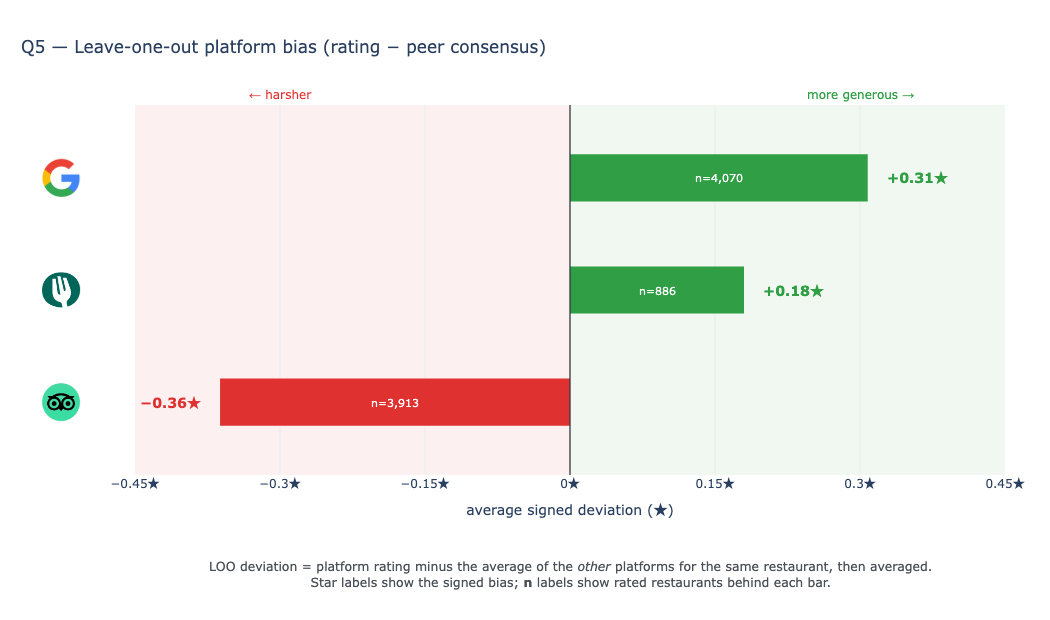
\includegraphics[width=\textwidth]{images/research_questions/q05_1.png}
\caption{Platform bias measured with a leave-one-out comparison. Values above zero indicate ratings higher than the other platforms; values below zero indicate lower ratings.}
\label{fig:rq-platform-bias}
\end{figure*}

\section{RQ2: Rating Level and Consistency by Cuisine}

Restaurant category affects both rating level and rating consistency.
Figure \ref{fig:rq-cuisine} compares cuisine types using the canonical taxonomy
produced after the cuisine reconciliation step. Pizza, fast-food and
American-style venues appear among the categories with lower average ratings and
larger cross-platform disagreement. By contrast, seafood, Japanese and African
cuisines are associated with higher and more consistent ratings. Rating level and
cross-platform agreement therefore tend to rise together: mainstream, high-volume
cuisines are both lower-rated and more contested, whereas specialist cuisines are
higher-rated and more aligned across platforms. The canonical
buckets make the pattern clearer than the older raw-label view and
remove the need to interpret separate labels such as \textit{Italiana} and
\textit{Italiano} as distinct cuisine groups.

\begin{figure*}[t]
\centering
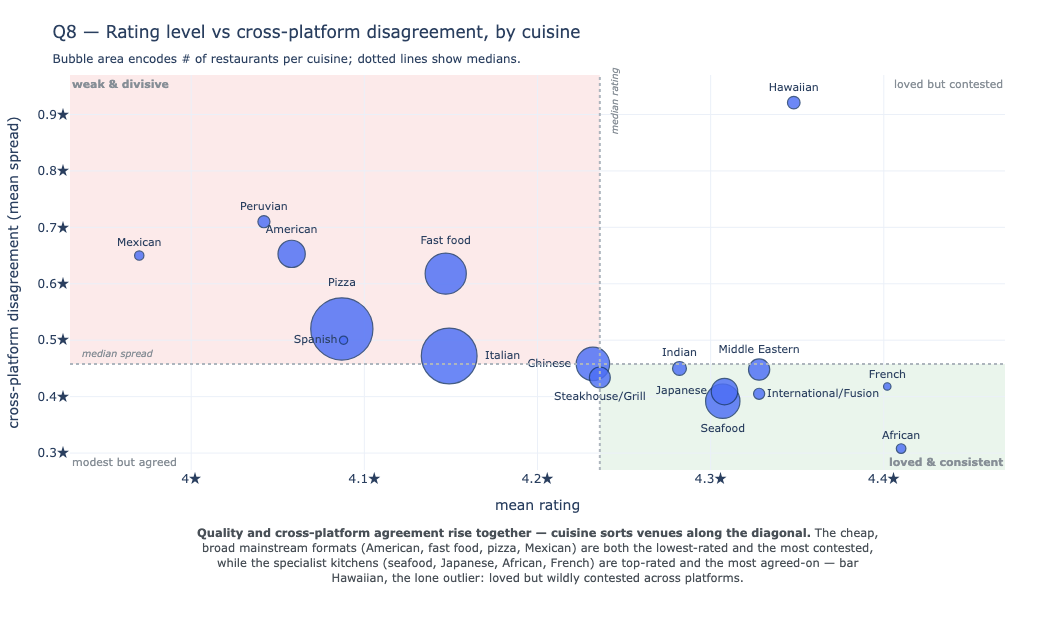
\includegraphics[width=\textwidth]{images/research_questions/q08_2.png}
\caption{Cuisine categories differ both in average rating and in rating disagreement across platforms.}
\label{fig:rq-cuisine}
\end{figure*}

\section{RQ3: Location and Data Completeness}

Location strongly affects data completeness. Completeness is quantified with a composite
score, defined as the mean presence rate over the platform-provided facets that
genuinely vary across the city: whether the restaurant has a website, whether it
carries a cuisine tag, and whether it is present on Tripadvisor and on TheFork. The
candidate signals were audited beforehand, and facets that are already saturated
everywhere, such as Google reviews, photos, and phone numbers, were excluded because
they do not discriminate between central and peripheral venues. The resulting score
is not distributed uniformly across Milan but depends strongly on where the
restaurant is located. Restaurants closer to the centre of the city are described
more completely. In the central area, the average number of platforms per restaurant
is 1.67, compared with 1.53 in the periphery.
Tripadvisor covers 53.1\% of central restaurants and 43.3\% of peripheral
restaurants; TheFork covers 13.9\% of central restaurants and 9.3\% of
peripheral restaurants. Central restaurants also have more Google reviews, with a
median of 269 compared with 161 in peripheral areas. Data completeness is
therefore spatially structured: central districts exhibit substantially richer
metadata than peripheral areas.

Figure \ref{fig:rq-coverage-density} makes this spatial completeness gradient
visible by mapping the composite completeness score across Milan. Each cell is
coloured by the average completeness of the venues it contains, from about 25\%
(dark blue) to about 65\% (light yellow). The historic core is data-rich, with
completeness above roughly 47\%, and completeness peaks in the Navigli and Isola
neighbourhoods before fading smoothly to around 30\% in the outer districts. The
map therefore confirms that the richest metadata is concentrated in the central
part of the city and decreases towards the periphery.

\begin{figure*}[t]
\centering
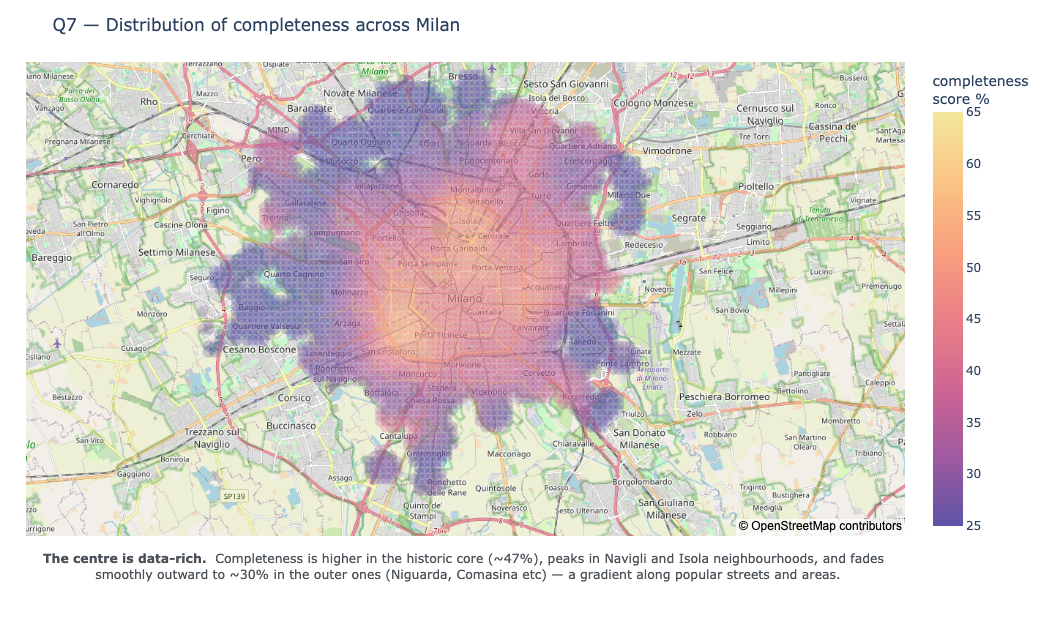
\includegraphics[width=\textwidth]{images/research_questions/q07_1.png}
\caption{Composite data-completeness score across Milan. Warmer colours indicate higher completeness; the score peaks in the historic centre and the Navigli/Isola belt and fades towards the periphery.}
\label{fig:rq-coverage-density}
\end{figure*}

\section{Further Analyses}
\label{sec:further-analyses}

The three research questions above are the focus of this report. The integrated
dataset is nonetheless designed to support a broader set of analytical questions,
which are explored in depth as part of the data-visualization module of the
course, including:

\begin{itemize}
\item How consistent are restaurant ratings across platforms overall?
\item Which restaurants exhibit the highest disagreement across platforms?
\item Is rating inconsistency linked to data-quality issues?
\item Can sparse, low-review data inflate perceived quality?
\item Does rating inconsistency rise for less popular venues?
\item Do pricier restaurants tend to rate higher and more consistently?
\item Are multi-platform venues rated differently?
\item Does photo richness track popularity or rating?
\end{itemize}

Each of these questions is backed by dedicated SQL over the ClickHouse analytical
tables and a corresponding notebook in the project repository, confirming that the
integrated schema is expressive enough to sustain them without any further data
collection.

\section{Summary}

Overall, the integrated database shows that online restaurant ratings in Milan
are usually similar across platforms, but not identical. Tripadvisor is
systematically more severe than Google and TheFork (RQ1); cuisine influences both
rating level and cross-platform agreement, with mainstream categories such as
pizza and fast food being lower-rated and more contested than specialist cuisines
(RQ2); and data completeness is spatially structured, with central districts
described far more richly than peripheral areas (RQ3). The integration of the
three sources therefore makes it possible to identify not only average restaurant
reputation, but also the cases where that reputation depends strongly on the
platform, the cuisine, and the location.
